\section{Results}
\label{sec:results}

\subsection{Deterministic degradation under missing history}
\label{sec:degradation}

The fixed-mask deterministic audit contains 48 dataset, mask-type, and missing-rate cells. Across the 12 dataset-by-mask-type curves, MSE increases monotonically over the evaluated missing rates. Table~\ref{tab:fixed-mask-degradation} gives the representative matrix retained in the main text, and Figure~\ref{fig:missingness-degradation} visualizes the degradation. The complete matrix appears in Appendix~\ref{app:additional-results}.

\begin{table}[t]
    \centering
    \caption{Forecast degradation under fixed historical masks. Relative degradation is measured against the corresponding clean TimePerceiver reference.}
    \label{tab:fixed-mask-degradation}
    \scriptsize
    \begin{tabular}{@{}lrrrr@{}}
\toprule
Dataset & Mask & Rate & MSE & Clean degradation \\
\midrule
ETTh1 & Block & 0.30 & 0.423837 & 13.19\% \\
ETTh1 & Channel & 0.30 & 0.583704 & 55.88\% \\
ETTh1 & Mixed & 0.30 & 0.495055 & 32.20\% \\
ETTh1 & Random & 0.10 & 0.378811 & 1.16\% \\
ETTh1 & Random & 0.30 & 0.425394 & 13.60\% \\
ETTh1 & Random & 0.50 & 0.525856 & 40.43\% \\
Electricity & Block & 0.30 & 0.184630 & 47.28\% \\
Electricity & Channel & 0.30 & 0.391038 & 211.92\% \\
Electricity & Mixed & 0.30 & 0.246785 & 96.86\% \\
Electricity & Random & 0.10 & 0.138429 & 10.42\% \\
Electricity & Random & 0.30 & 0.200572 & 59.99\% \\
Electricity & Random & 0.50 & 0.325732 & 159.83\% \\
Weather & Block & 0.30 & 0.180420 & 25.24\% \\
Weather & Channel & 0.30 & 0.284471 & 97.47\% \\
Weather & Mixed & 0.30 & 0.224939 & 56.14\% \\
Weather & Random & 0.10 & 0.169631 & 17.75\% \\
Weather & Random & 0.30 & 0.240810 & 67.16\% \\
Weather & Random & 0.50 & 0.331313 & 129.99\% \\
\bottomrule
\end{tabular}

\end{table}

\begin{figure}[t]
    \centering
    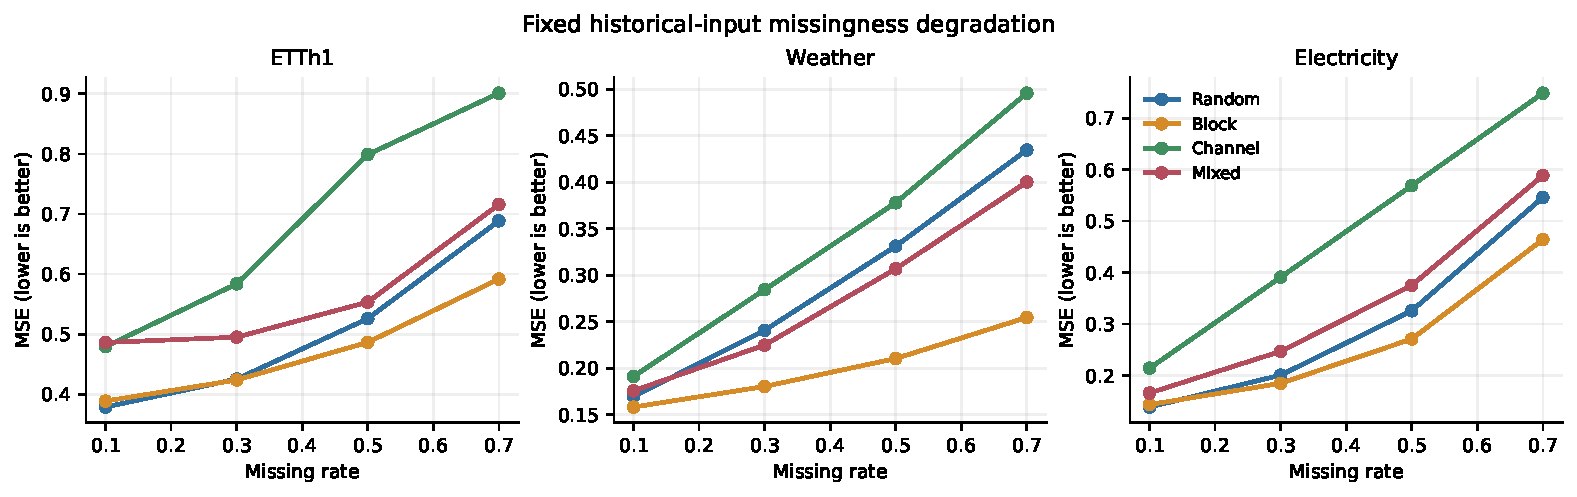
\includegraphics[width=0.96\linewidth]{figures/fig1_missingness_degradation.pdf}
    \caption{MSE under the fixed missing-history evaluation. Higher missing rates increase error across the evaluated datasets and mask types.}
    \label{fig:missingness-degradation}
\end{figure}

\subsection{TimePerceiver probabilistic forecasting}
\label{sec:timeperceiver-results}

The primary TimePerceiver matrix contains 12 paired cells: three datasets crossed with four probability-head training seeds. Student-$t$ variants record 12/12 NLL wins, 12/12 CRPS-noninferior outcomes, 12/12 point-noninferior outcomes, and 12/12 full paired passes. All 3/3 dataset-level mean gates pass. Table~\ref{tab:timeperceiver-multiseed} reports the dataset means and standard deviations.

\begin{table}[t]
    \centering
    \caption{TimePerceiver four-head-seed comparison. Deltas are Student-$t$ minus Gaussian; negative values favor Student-$t$.}
    \label{tab:timeperceiver-multiseed}
    \scriptsize
    \resizebox{\linewidth}{!}{\begin{tabular}{@{}lrrrrrrrrrrr@{}}
\toprule
Dataset & G NLL & T NLL & $\Delta$NLL & NLL wins & G CRPS & T CRPS & $\Delta$CRPS & G MSE & T MSE & $\Delta$MSE & Point NI \\
\midrule
ETTh1 & 0.915014 & 0.871113 & -0.043900 & 4 & 0.342011 & 0.337656 & -0.004356 & 0.416862 & 0.415611 & -0.001252 & 4 \\
Weather & 0.577226 & 0.103670 & -0.473557 & 4 & 0.244788 & 0.207544 & -0.037245 & 0.210306 & 0.209818 & -0.000488 & 4 \\
Electricity & 0.439644 & 0.365348 & -0.074296 & 4 & 0.209365 & 0.207395 & -0.001970 & 0.167419 & 0.167703 & 0.000284 & 4 \\
\bottomrule
\end{tabular}
}
\end{table}

Figure~\ref{fig:multiseed-nll-deltas} shows paired NLL changes for every dataset and seed. Figure~\ref{fig:multiseed-summary} summarizes NLL, CRPS, and MSE means. The evidence concerns probability-head optimization on fixed official backbone checkpoints, so it does not measure variability from backbone retraining.

\begin{figure}[t]
    \centering
    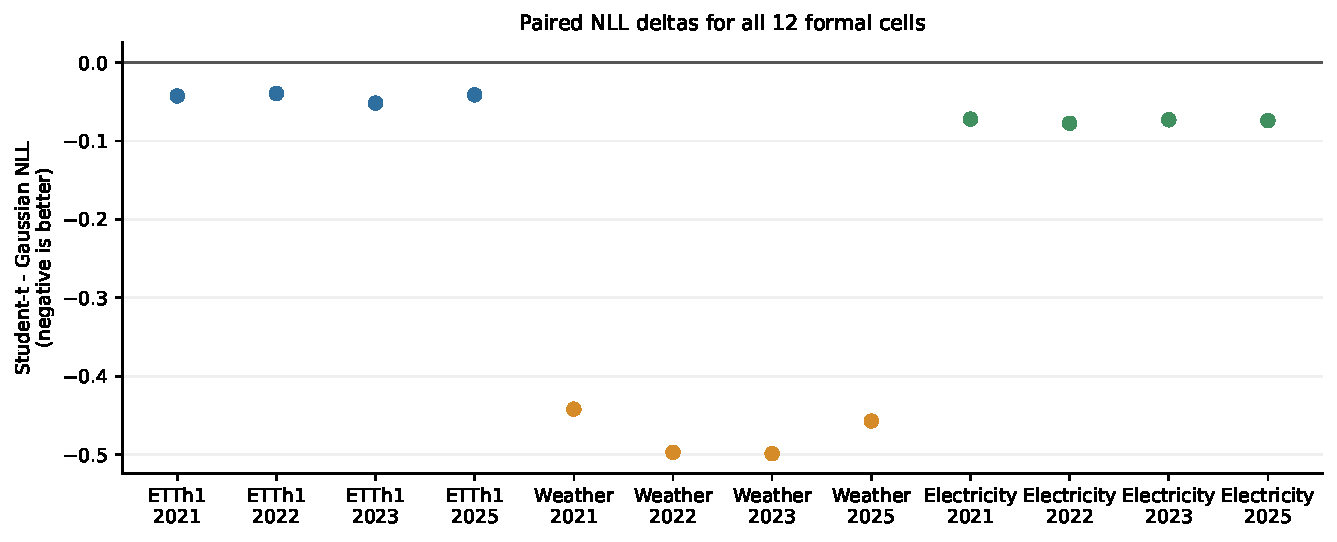
\includegraphics[width=0.96\linewidth]{figures/fig2_multiseed_nll_deltas.pdf}
    \caption{Paired NLL deltas for the TimePerceiver multi-seed matrix. Every displayed delta is negative.}
    \label{fig:multiseed-nll-deltas}
\end{figure}

\begin{figure}[t]
    \centering
    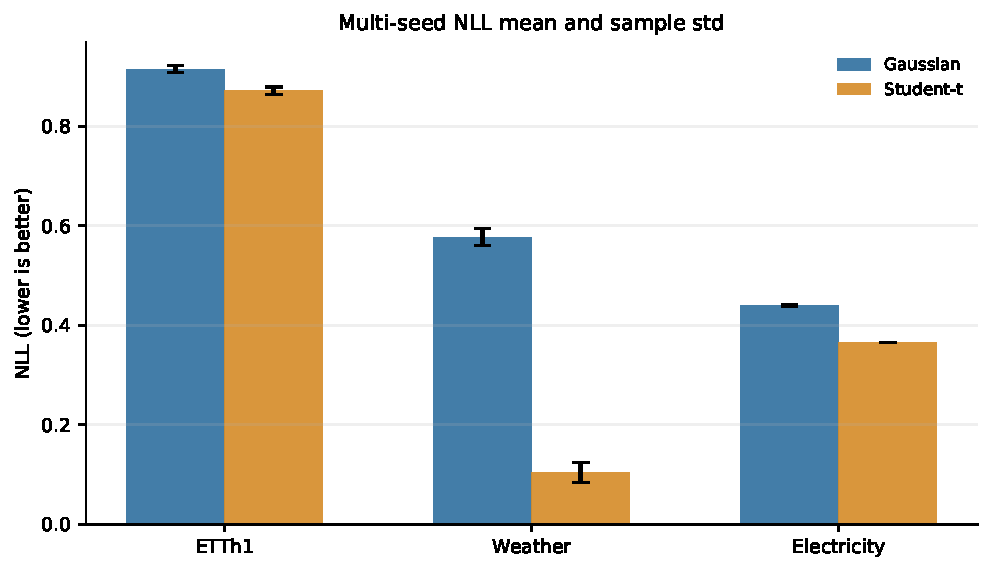
\includegraphics[width=0.32\linewidth]{figures/fig3a_multiseed_nll.pdf}
    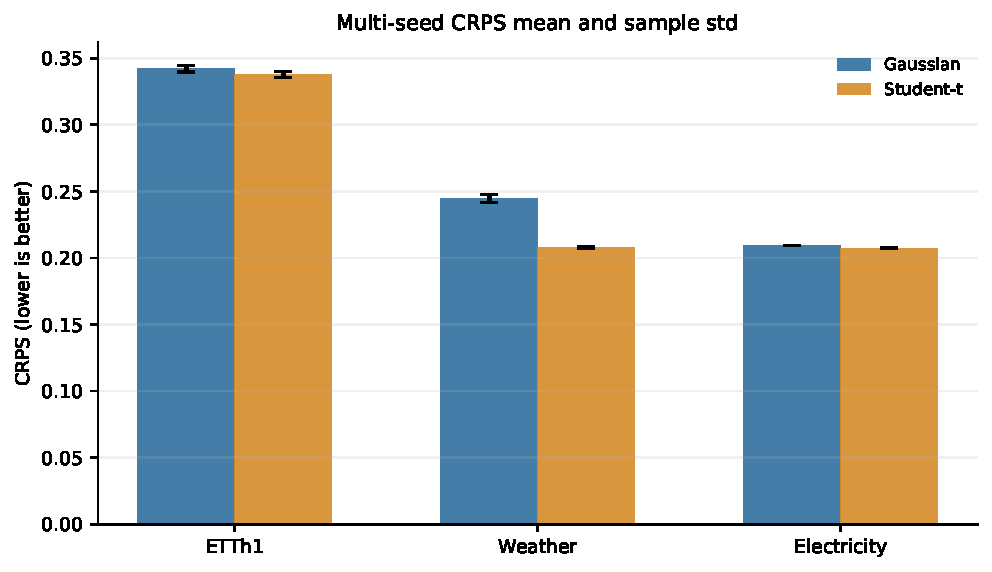
\includegraphics[width=0.32\linewidth]{figures/fig3b_multiseed_crps.pdf}
    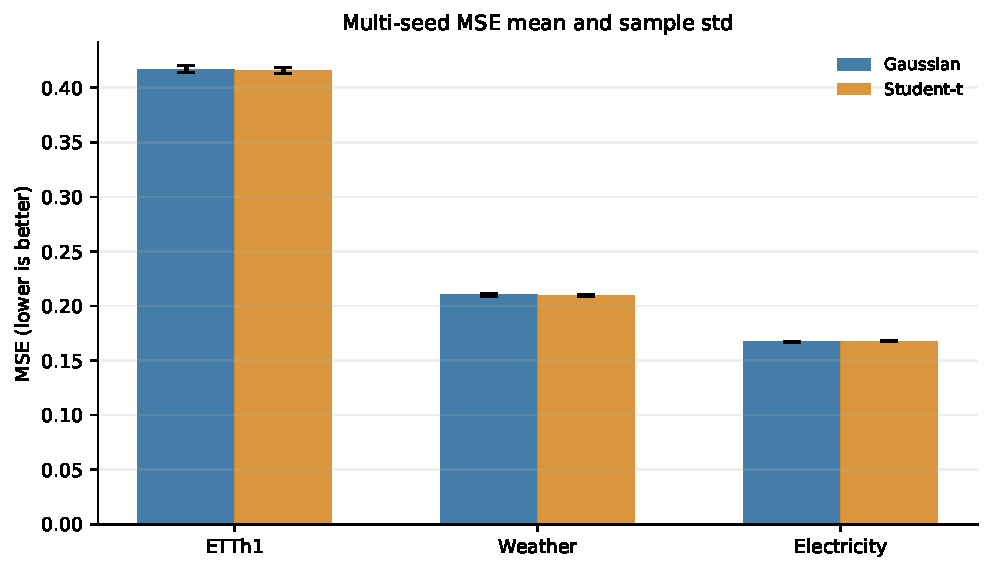
\includegraphics[width=0.32\linewidth]{figures/fig3c_multiseed_mse.pdf}
    \caption{TimePerceiver dataset-level mean and standard-deviation summaries for NLL, CRPS, and MSE across four probability-head training seeds.}
    \label{fig:multiseed-summary}
\end{figure}

\subsection{Distribution-head ablation}
\label{sec:distribution-ablation}

Table~\ref{tab:distribution-ablation} compares Gaussian, Laplace, fixed Student-$t$, and learned-df Student-$t$ heads under random missingness at rate 0.3. The fixed Student-$t$ head records 3/3 NLL wins, 3/3 CRPS-noninferior outcomes, and 3/3 point-noninferior outcomes against Gaussian. The learned-df variant does not consistently improve over fixed df=8. Laplace also lacks equal support across all paired criteria. The formal conclusion is therefore that a fixed heavy-tailed likelihood is sufficient in the evaluated scope.

\begin{table}[t]
    \centering
    \caption{Distribution-head ablation on frozen TimePerceiver checkpoints. The fixed Student-$t$ head uses df=8.}
    \label{tab:distribution-ablation}
    \scriptsize
    \resizebox{\linewidth}{!}{\begin{tabular}{@{}lrrrrrr@{}}
\toprule
Dataset & Head & NLL & CRPS & MSE & Coverage error & Trainable \\
\midrule
etth1 & Gaussian & 0.918535 & 0.344127 & 0.420332 & 0.038132 & 6,168 \\
etth1 & Laplace & 0.879116 & 0.341785 & 0.424149 & 0.011910 & 6,168 \\
etth1 & Fixed Student-t (df=8) & 0.864949 & 0.336548 & 0.413927 & 0.022006 & 6,168 \\
etth1 & Learned Student-t & 0.877154 & 0.340263 & 0.419177 & 0.020301 & 6,175 \\
weather & Gaussian & 0.586325 & 0.245442 & 0.212237 & 0.082667 & 24,624 \\
weather & Laplace & 0.204399 & 0.209589 & 0.210051 & 0.070806 & 24,624 \\
weather & Fixed Student-t (df=8) & 0.136165 & 0.208461 & 0.210994 & 0.051632 & 24,624 \\
weather & Learned Student-t & 0.129293 & 0.208276 & 0.210836 & 0.052156 & 24,645 \\
electricity & Gaussian & 0.440598 & 0.209453 & 0.167881 & 0.038304 & 24,624 \\
electricity & Laplace & 0.370388 & 0.208768 & 0.170436 & 0.018222 & 24,624 \\
electricity & Fixed Student-t (df=8) & 0.367009 & 0.207797 & 0.168473 & 0.018744 & 24,624 \\
electricity & Learned Student-t & 0.366449 & 0.207786 & 0.168486 & 0.018502 & 24,945 \\
\bottomrule
\end{tabular}
}
\end{table}

The fixed Student-$t$ head has the same trainable parameter count as Gaussian and Laplace. Table~\ref{tab:efficiency} reports the controlled parameter, latency, and memory measurements. The learned-df head adds only per-channel shape parameters, yet this extra flexibility does not produce a consistent metric benefit.

\begin{table}[t]
    \centering
    \caption{Controlled probability-head efficiency measurements. Timing comparisons are within each dataset and benchmark environment.}
    \label{tab:efficiency}
    \scriptsize
    \resizebox{\linewidth}{!}{\begin{tabular}{@{}lrrrrrr@{}}
\toprule
Dataset & Head & Params & Forward ms & NLL ms & CRPS ms & Peak MiB \\
\midrule
etth1 & Gaussian & 6,168 & 29.997997 & 51.514500 & 86.934799 & 215.033691 \\
etth1 & Laplace & 6,168 & 29.996887 & 30.016349 & 63.189127 & 215.033691 \\
etth1 & Fixed Student-t (df=8) & 6,168 & 29.902914 & 65.900001 & 90.256716 & 215.034180 \\
etth1 & Learned Student-t & 6,175 & 29.982518 & 69.371223 & 103.335362 & 215.034180 \\
weather & Gaussian & 24,624 & 59.357760 & 79.919755 & 188.685383 & 630.664551 \\
weather & Laplace & 24,624 & 58.485584 & 59.293318 & 133.341993 & 630.664551 \\
weather & Fixed Student-t (df=8) & 24,624 & 58.181018 & 98.037041 & 211.123562 & 630.665039 \\
weather & Learned Student-t & 24,645 & 59.026097 & 97.896011 & 212.516092 & 630.665039 \\
electricity & Gaussian & 24,624 & 356.894562 & 359.007118 & 1248.479182 & 4626.902832 \\
electricity & Laplace & 24,624 & 345.290164 & 343.346301 & 895.849843 & 4626.902832 \\
electricity & Fixed Student-t (df=8) & 24,624 & 343.877731 & 374.742924 & 1477.667372 & 4626.904297 \\
electricity & Learned Student-t & 24,945 & 420.384170 & 473.496327 & 1890.070674 & 4626.904297 \\
\bottomrule
\end{tabular}
}
\end{table}

\subsection{Second-backbone replication}
\label{sec:patchtst-results}

The PatchTST comparison records 3/3 NLL wins, 3/3 CRPS-noninferior outcomes, 2/3 point-noninferior outcomes, and 2/3 full paired passes for the fixed Student-$t$ head. Table~\ref{tab:second-backbone} reports the paired deltas, and Figure~\ref{fig:cross-backbone-deltas} visualizes their signs. ETTh1 and Weather pass every component.

Electricity does not pass the point criterion. Gaussian MSE is 0.165829 and fixed Student-$t$ MSE is 0.167809, a change of +0.001980 or +1.194\%. The increase is above the pre-registered 1\% tolerance in Equation~\ref{eq:point-gate}. The decision is therefore \texttt{SECOND\_BACKBONE\_POINT\_TRADEOFF}. The NLL and CRPS direction transfers to PatchTST, but the complete multi-metric gate does not.

\begin{table}[t]
    \centering
    \caption{Within-backbone deltas for fixed Student-$t$ versus Gaussian. The point threshold permits at most a 1\% relative MSE increase.}
    \label{tab:second-backbone}
    \scriptsize
    \resizebox{\linewidth}{!}{\begin{tabular}{@{}lrrrrrrrrr@{}}
\toprule
Dataset & Backbone & $\Delta$NLL & $\Delta$CRPS & $\Delta$MSE & Rel. MSE & NLL win & CRPS NI & Point NI & Full pair \\
\midrule
ETTh1 & TimePerceiver & -0.053587 & -0.007578 & -0.006405 & -1.524\% & Yes & Yes & Yes & Yes \\
ETTh1 & PatchTST & -0.035317 & -0.002538 & -0.005439 & -1.274\% & Yes & Yes & Yes & Yes \\
Weather & TimePerceiver & -0.450160 & -0.036981 & -0.001243 & -0.586\% & Yes & Yes & Yes & Yes \\
Weather & PatchTST & -1.818698 & -0.076205 & -0.050179 & -21.595\% & Yes & Yes & Yes & Yes \\
Electricity & TimePerceiver & -0.073589 & -0.001656 & 0.000592 & +0.353\% & Yes & Yes & Yes & Yes \\
Electricity & PatchTST & -0.083433 & -0.001688 & 0.001980 & +1.194\% & Yes & Yes & No & No \\
\bottomrule
\end{tabular}
}
\end{table}

\begin{figure}[t]
    \centering
    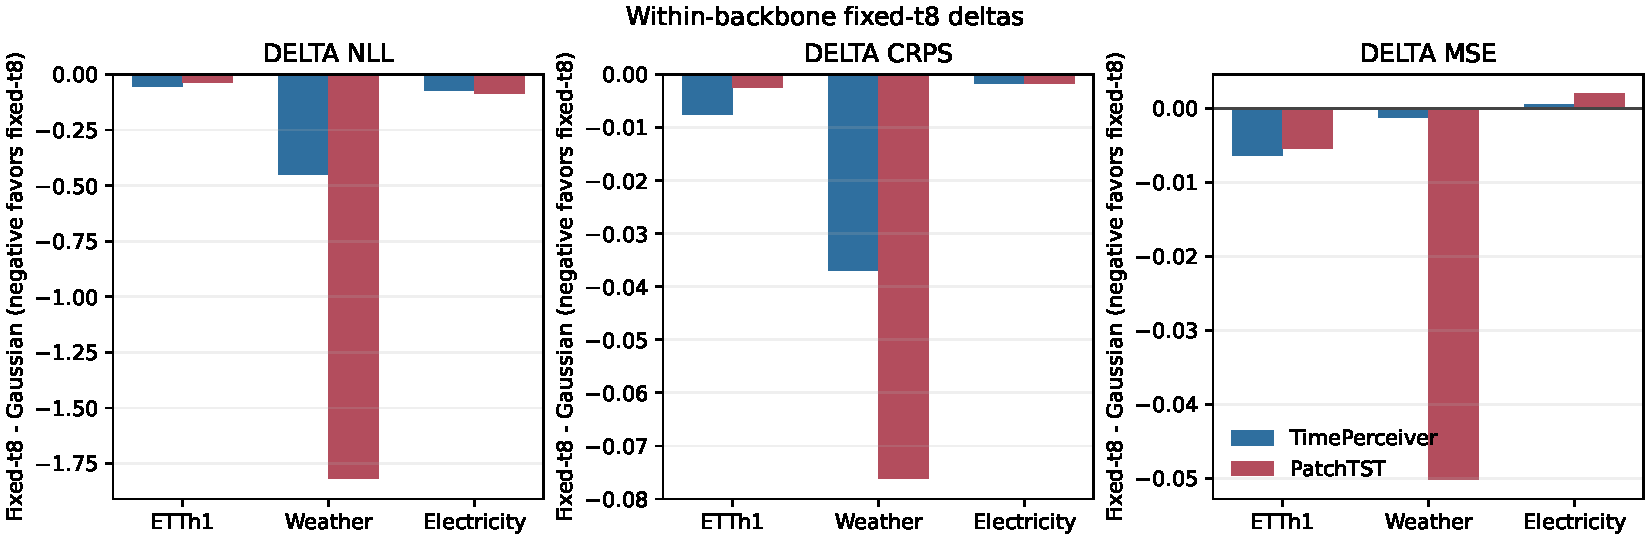
\includegraphics[width=0.96\linewidth]{figures/fig_gate5b_cross_backbone_deltas.pdf}
    \caption{Within-backbone metric deltas. Negative values favor the fixed Student-$t$ head. PatchTST NLL and CRPS improve on all three datasets, while Electricity has a small positive MSE delta.}
    \label{fig:cross-backbone-deltas}
\end{figure}

\subsection{Heavy-tail diagnostics}
\label{sec:tail-diagnostics}

Residual-percentile diagnostics indicate that much of the NLL gain appears in the most extreme Gaussian-residual region. Figure~\ref{fig:tail-nll} shows this pattern for the TimePerceiver ablation. The corresponding PatchTST diagnostic covers approximately $1.82\times10^8$ forecast elements and yields the same qualitative concentration in its most extreme bin. These analyses are descriptive. They are not formal gate evidence, causal mechanism tests, or inferential samples of $1.82\times10^8$ independent observations.

\begin{figure}[t]
    \centering
    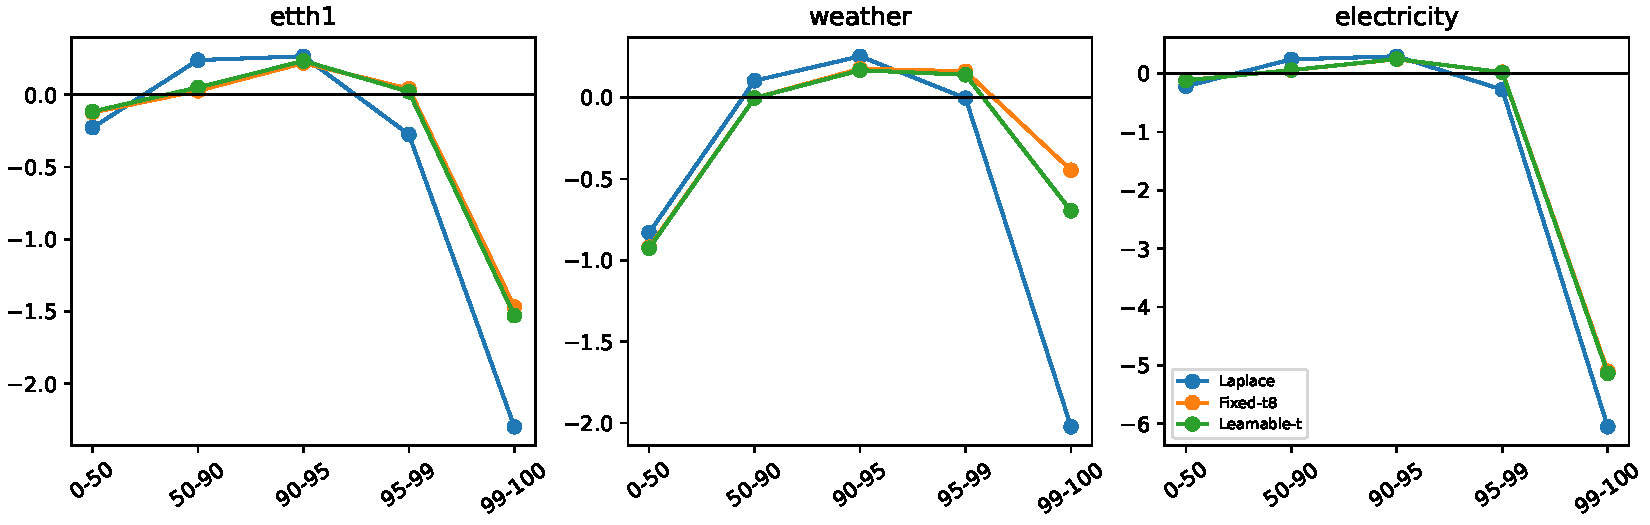
\includegraphics[width=0.90\linewidth]{figures/fig_gate5a_tail_nll_gain.pdf}
    \caption{Descriptive NLL differences across Gaussian-residual percentile bins for the TimePerceiver distribution ablation.}
    \label{fig:tail-nll}
\end{figure}
